\begin{exo}
	Soit $ABCD$ un rectangle de centre $O$ dont la longueur est le double de la largeur.

	On note $R$ le milieu du segment $[AB]$, $P$ le milieu du segment $[OC]$ et $Q$ un point du segment $[BC]$ tel que $BQ = \frac{1}{4}BC$.

	L'objectif de l'exercice est de déterminer l'aire du quadrilatère $OPQR$.
	\begin{center}
		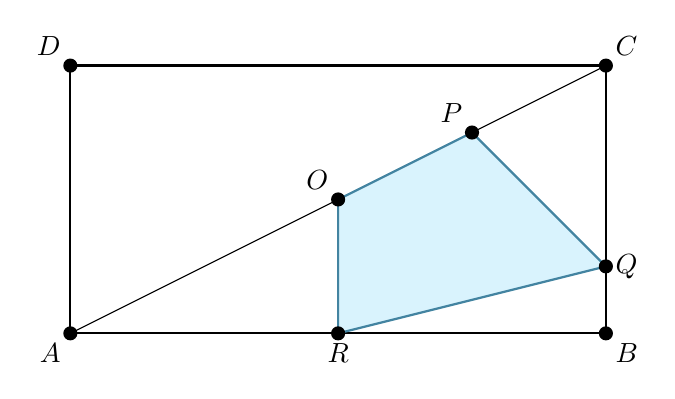
\begin{tikzpicture}[scale=1.7]
			\coordinate (A) at (0,0);
			\coordinate (B) at (4,0);
			\coordinate (C) at (4,2);
			\coordinate (D) at (0,2);
			\coordinate (R) at (2,0);
			\coordinate (O) at (2,1);
			\coordinate (P) at (3,1.5);
			\coordinate (Q) at (4,0.5);
			\draw[thick] (A) -- (B) -- (C) -- (D) -- cycle;
			\draw (A) -- (C);
			\draw[thick, cyan!60!black, fill=cyan!15] (O) -- (P) -- (Q) -- (R) -- cycle;
			\foreach \p/\pos in {A/below left, B/below right, C/above right, D/above left, O/above left, R/below, P/above left, Q/right} { \node[\pos] at (\p) {$\p$}; }
			\fill (A) circle (1.5pt);
			\fill (B) circle (1.5pt);
			\fill (C) circle (1.5pt);
			\fill (D) circle (1.5pt);
			\fill (O) circle (1.5pt);
			\fill (R) circle (1.5pt);
			\fill (P) circle (1.5pt);
			\fill (Q) circle (1.5pt);
		\end{tikzpicture}
	\end{center}

	On considère le repère $(A;R,D)$.

	\begin{enumerate}
		\item Expliquer pourquoi le repère $(A;R,D)$ est un repère orthonormé du plan.
		\item Donner, sans justification, les coordonnées des points $A$, $B$, $C$, $R$ et $Q$.
		\item Calculer $AB$ et $CB$.

		      En déduire l'aire du triangle $ABC$.
		\item Calculer $BR$ et $BQ$.

		      En déduire l'aire du triangle $BQR$.
		\item Calculer les coordonnées des points $O$ et $P$.
		\item Calculer l'aire du triangle $ARO$.
		\item On note $H$ le projeté orthogonal de $P$ sur $(BC)$. On admet que $H$ a pour coordonnées $\coordl{2}{\frac{3}{4}}$.
		      \begin{enumerate}
			      \item Calculer $HP$.

			            En déduire l'aire du triangle $CQP$.
			      \item En déduire l'aire du quadrilatère $OPQR$.
		      \end{enumerate}
	\end{enumerate}
\end{exo}
